% Keypoint R-CNN as actually configured here: ResNet-50 + FPN backbone, RPN proposals,
% RoIAlign to 14x14, eight 3x3 convolutions, two deconv/upsample stages to a 56x56
% heatmap per keypoint, spatial argmax to coordinates. K = 2 per head, three heads.
\documentclass[border=8pt,multi,tikz]{standalone}
\usepackage{amsmath}
\usepackage{helvet}
\renewcommand{\familydefault}{\sfdefault}
\usetikzlibrary{positioning,arrows.meta,calc,fit,backgrounds,shapes.geometric,
                decorations.pathreplacing,patterns}

\definecolor{ink}{HTML}{1D2433}
\definecolor{muted}{HTML}{6B7280}
\definecolor{accent}{HTML}{D62828}
\definecolor{good}{HTML}{2A9D8F}
\definecolor{soft}{HTML}{E8ECF1}
\definecolor{edge}{HTML}{AAB3C0}
\definecolor{bb}{HTML}{4C6EF5}
\definecolor{fpn}{HTML}{7048E8}
\definecolor{headc}{HTML}{0CA678}

\begin{document}
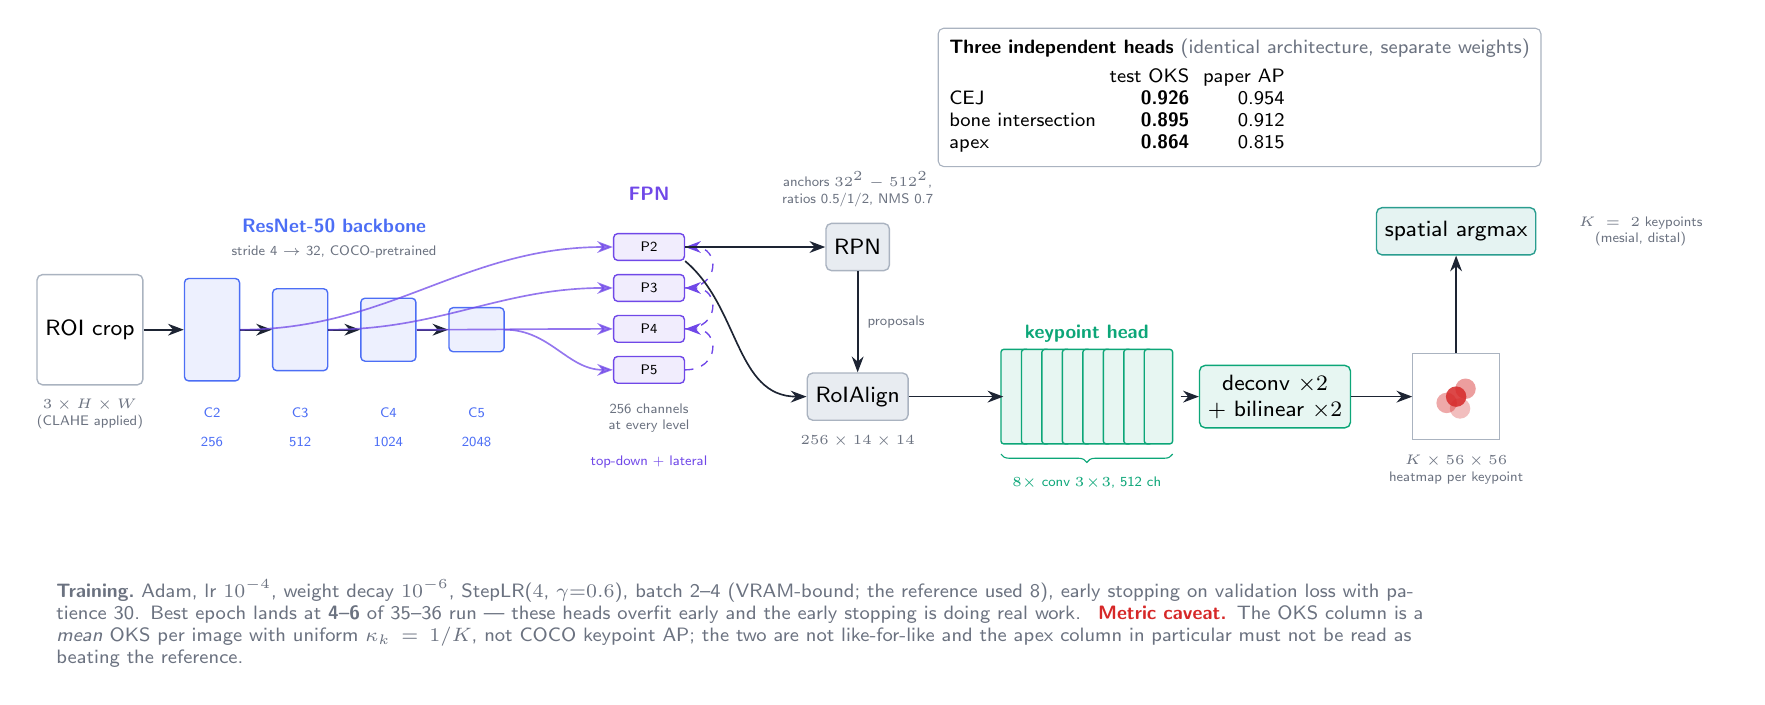
\begin{tikzpicture}[
  font=\sffamily\footnotesize,
  >={Stealth[length=2mm]},
  stage/.style={draw=edge,fill=soft,rounded corners=2pt,minimum height=6mm,
                align=center,inner xsep=3pt,line width=0.5pt},
  conv/.style={draw=headc,fill=headc!10,rounded corners=1pt,minimum width=3.6mm,
               minimum height=12mm,inner sep=0pt,line width=0.5pt},
  lbl/.style={font=\sffamily\scriptsize,text=muted,align=center},
  tiny/.style={font=\sffamily\tiny,text=muted,align=center},
  tag/.style={font=\sffamily\bfseries\scriptsize,text=ink},
  fl/.style={->,draw=ink,line width=0.6pt},
]

%---------------------------------------------------------------- input ---
\node[stage,fill=white,minimum height=14mm,minimum width=13mm] (roi) at (0,0)
  {ROI crop};
\node[tiny,below=0.5mm of roi] {$3\times H\times W$\\(CLAHE applied)};

%--------------------------------------------------------- ResNet-50 stages ---
\foreach \i/\nm/\ch/\h in {1/C2/256/13, 2/C3/512/10.4, 3/C4/1024/8, 4/C5/2048/5.6}{
  \pgfmathsetmacro{\xx}{1.55+(\i-1)*1.12}
  \node[draw=bb,fill=bb!10,rounded corners=1.5pt,minimum width=7mm,
        minimum height=\h mm,inner sep=0pt,line width=0.5pt] (\nm) at (\xx,0) {};
  \node[tiny,text=bb] at (\xx,-1.05) {\nm};
  \node[tiny,text=bb] at (\xx,-1.42) {\ch};
}
\node[tag,text=bb] at (3.1,1.32) {ResNet-50 backbone};
\node[tiny] at (3.1,0.98) {stride 4 $\to$ 32, COCO-pretrained};

\draw[fl] (roi.east) -- (C2.west);
\foreach \a/\b in {C2/C3,C3/C4,C4/C5}{\draw[fl] (\a) -- (\b);}

%-------------------------------------------------------------------- FPN ---
\foreach \i/\nm in {1/P2, 2/P3, 3/P4, 4/P5}{
  \pgfmathsetmacro{\yy}{1.05-(\i-1)*0.52}
  \node[draw=fpn,fill=fpn!10,rounded corners=1.5pt,minimum width=9mm,
        minimum height=3.4mm,inner sep=0pt,line width=0.5pt] (\nm) at (7.1,\yy) {\tiny\nm};
}
\node[tag,text=fpn] at (7.1,1.72) {FPN};
\node[tiny] at (7.1,-1.12) {256 channels\\at every level};

\foreach \c/\p in {C2/P2, C3/P3, C4/P4, C5/P5}{
  \draw[fl,draw=fpn,opacity=0.75] (\c.east) to[out=0,in=180] (\p.west);}
\foreach \a/\b in {P5/P4, P4/P3, P3/P2}{
  \draw[->,draw=fpn,dashed,line width=0.5pt] (\a.east) to[out=0,in=0,looseness=2.2] (\b.east);}
\node[tiny,text=fpn] at (7.10,-1.68) {top-down + lateral};

%-------------------------------------------------------------------- RPN ---
\node[stage,draw=edge] (rpn) at (9.75,1.05) {RPN};
\node[tiny,above=0.8mm of rpn,text width=32mm]
  {anchors $32^2\!-\!512^2$, ratios 0.5/1/2, NMS 0.7};
\draw[fl] (P2.east) to[out=0,in=180] (rpn.west);

%--------------------------------------------------------------- RoIAlign ---
\node[stage] (roial) at (9.75,-0.85) {RoIAlign};
\node[tiny,below=0.6mm of roial] {$256\times14\times14$};
\draw[fl] (rpn.south) -- node[right,tiny]{proposals} (roial.north);
\draw[fl] (P2.south east) to[out=-40,in=180] (roial.west);

%------------------------------------------------------------ keypoint head ---
\begin{scope}[xshift=11.45cm]
  \foreach \i in {1,...,8}{
    \pgfmathsetmacro{\xx}{0.30+(\i-1)*0.26}
    \node[conv] (k\i) at (\xx,-0.85) {};
  }
  \draw[decorate,decoration={brace,amplitude=3pt,mirror},draw=headc]
    (0.12,-1.58) -- (2.30,-1.58);
  \node[tiny,text=headc] at (1.21,-1.95) {$8\times$ conv $3\!\times\!3$, 512 ch};
  \node[tag,text=headc] at (1.21,-0.05) {keypoint head};
\end{scope}
\draw[fl] (roial.east) -- (11.60,-0.85);

%------------------------------------------------------- deconv + heatmap ---
\node[stage,draw=headc,fill=headc!10] (deconv) at (15.05,-0.85)
  {deconv $\times2$\\+ bilinear $\times2$};
\draw[fl] (13.85,-0.85) -- (deconv.west);

\node[draw=edge,fill=white,minimum width=11mm,minimum height=11mm,inner sep=0pt]
  (hm) at (17.35,-0.85) {};
\foreach \x/\y/\o in {0.0/0.0/0.85, 0.12/0.1/0.45, -0.12/-0.08/0.4, 0.05/-0.15/0.3}{
  \fill[accent,opacity=\o] ($(hm.center)+(\x,\y)$) circle (0.13);}
\node[tiny,below=0.6mm of hm] {$K\times56\times56$\\heatmap per keypoint};
\draw[fl] (deconv.east) -- (hm.west);

\node[stage,fill=good!12,draw=good] (arg) at (17.35,1.25) {spatial argmax};
\node[tiny,right=1mm of arg,text width=22mm] {$K=2$ keypoints\\(mesial, distal)};
\draw[fl] (hm.north) -- (arg.south);

%------------------------------------------------------------------ heads ---
\node[draw=edge,fill=white,rounded corners=2pt,align=left,inner sep=4pt,
      font=\sffamily\scriptsize] (three) at (14.6,2.95)
  {\textbf{Three independent heads} \textcolor{muted}{(identical architecture, separate weights)}\\[2pt]
   \begin{tabular}{@{}l@{\ \ }r@{\ \ }r@{}}
   & \scriptsize test OKS & \scriptsize paper AP\\
   CEJ & \textbf{0.926} & 0.954\\
   bone intersection & \textbf{0.895} & 0.912\\
   apex & \textbf{0.864} & 0.815\\
   \end{tabular}};

%------------------------------------------------------------------ notes ---
\node[anchor=north west,font=\sffamily\scriptsize,text=muted,text width=176mm]
  at (-0.55,-3.05)
  {\textbf{Training.}\ Adam, lr $10^{-4}$, weight decay $10^{-6}$, StepLR($4$, $\gamma{=}0.6$),
   batch 2--4 (VRAM-bound; the reference used 8), early stopping on validation loss with
   patience 30. Best epoch lands at \textbf{4--6} of 35--36 run --- these heads overfit early and
   the early stopping is doing real work.
   \ \textbf{\textcolor{accent}{Metric caveat.}} The OKS column is a \emph{mean} OKS per image with
   uniform $\kappa_k=1/K$, not COCO keypoint AP; the two are not like-for-like and the apex
   column in particular must not be read as beating the reference.};

\end{tikzpicture}
\end{document}
